% this TeX file provides an awesome example of how TeX will make super 
% awesome tables, at the cost of your of what happens when you try to make a
% table that is very complicated.
\documentclass[11pt]{article}

% Use wide margins, but not quite so wide as fullpage.sty
\marginparwidth 0.5in 
\oddsidemargin 0.25in 
\evensidemargin 0.25in 
\marginparsep 0.25in
\topmargin 0.25in
\textwidth 6in
\textheight 8in
% That's about enough definitions

% language input
\usepackage[utf8]{inputenc}
% multirow allows you to combine rows in columns
\usepackage{multirow}
% tabularx allows manual tweaking of column width
\usepackage{tabularx}
% insert images
\usepackage{graphicx}
\usepackage{float}
\graphicspath{ {images/} }

\begin{document}
% this is an alternate method of creating a title
%\hfill\vbox{\hbox{Gius, Mark}
%       \hbox{Cpe 456, Section 01}  
%       \hbox{Lab 1}    
%       \hbox{\today}}\par
%
%\bigskip
%\bigskip
\author{Vandré Leal Cândido}
\title{Wireshark Lab: UDP v6.1}
\maketitle

%\begin{figure}[H]
%\centering
%\caption{Request (Section 1)}
%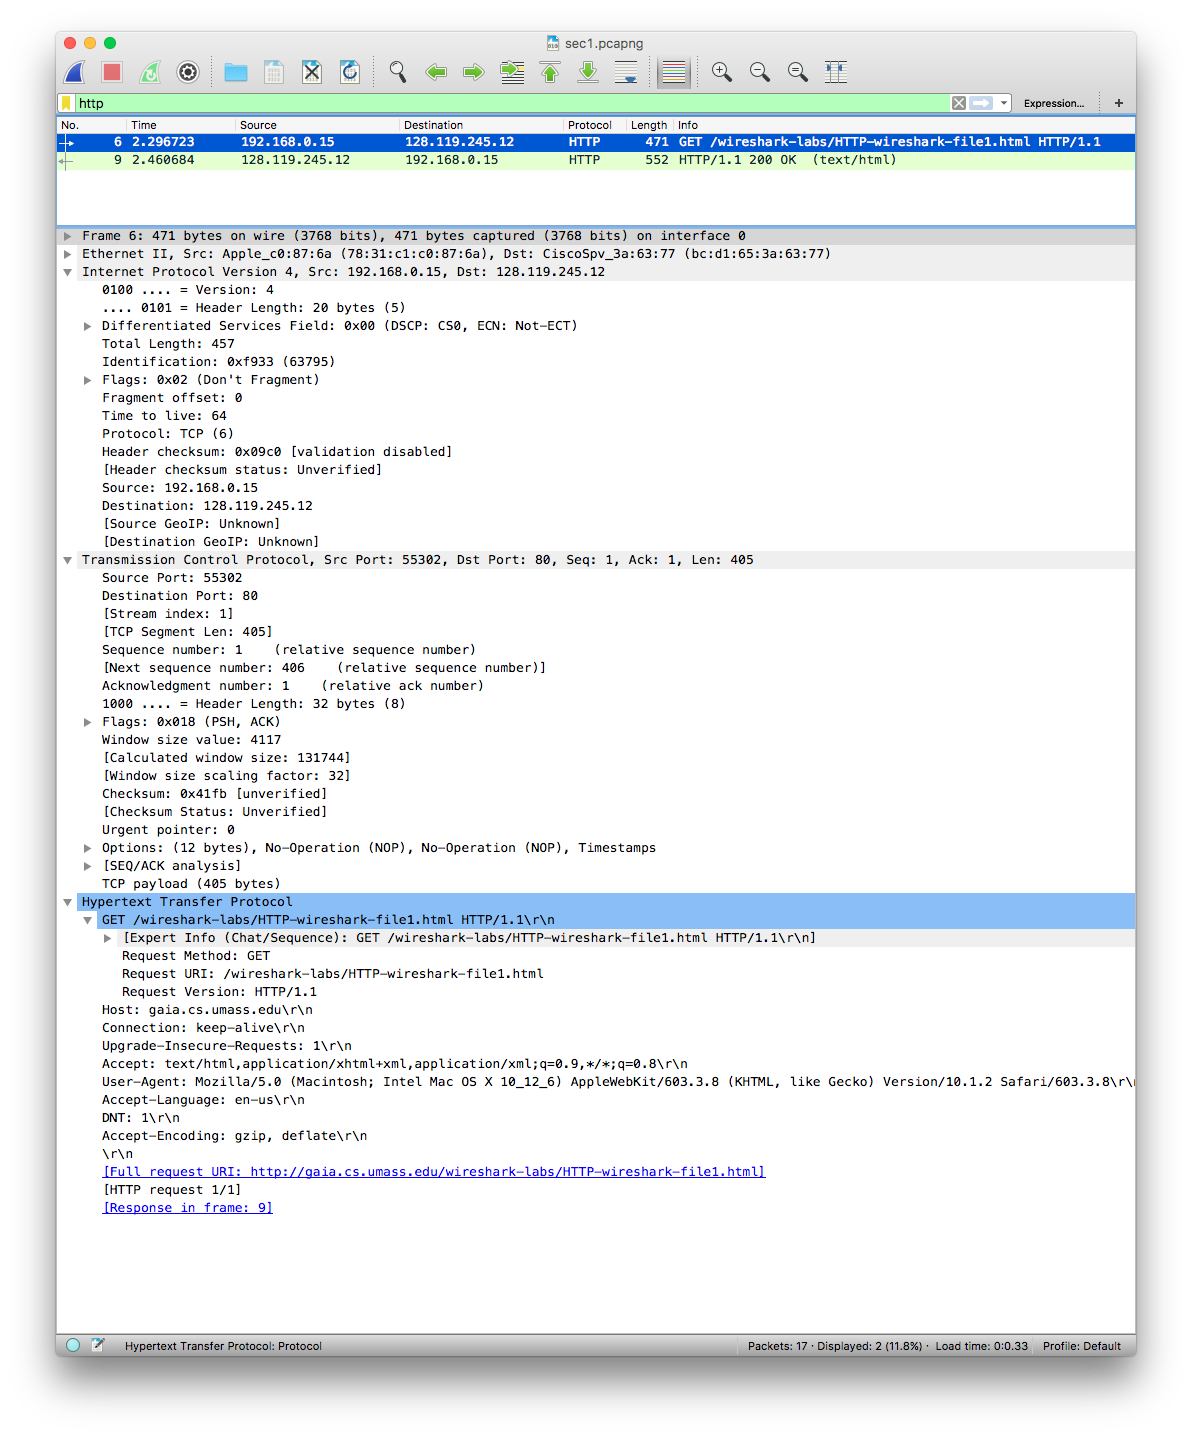
\includegraphics[width=\textwidth]{01-request}
%\end{figure}

% The Assignment
\section{The Assignment}

\begin{itemize}
	\setlength\itemsep{.5cm}

	\item
		\textit{Select one UDP packet from your trace. From this packet, determine how many fields there are in the UDP header. (You shouldn’t look in the textbook! Answer these questions directly from what you observe in the packet trace.) Name these fields.}
		\par There are four fields in the UDP header: \textbf{Source Port}, \textbf{Destination Port}, \textbf{Length} and \textbf{Checksum}.
		
		\begin{figure}[H]
		\centering
		\caption{UDP packet}
		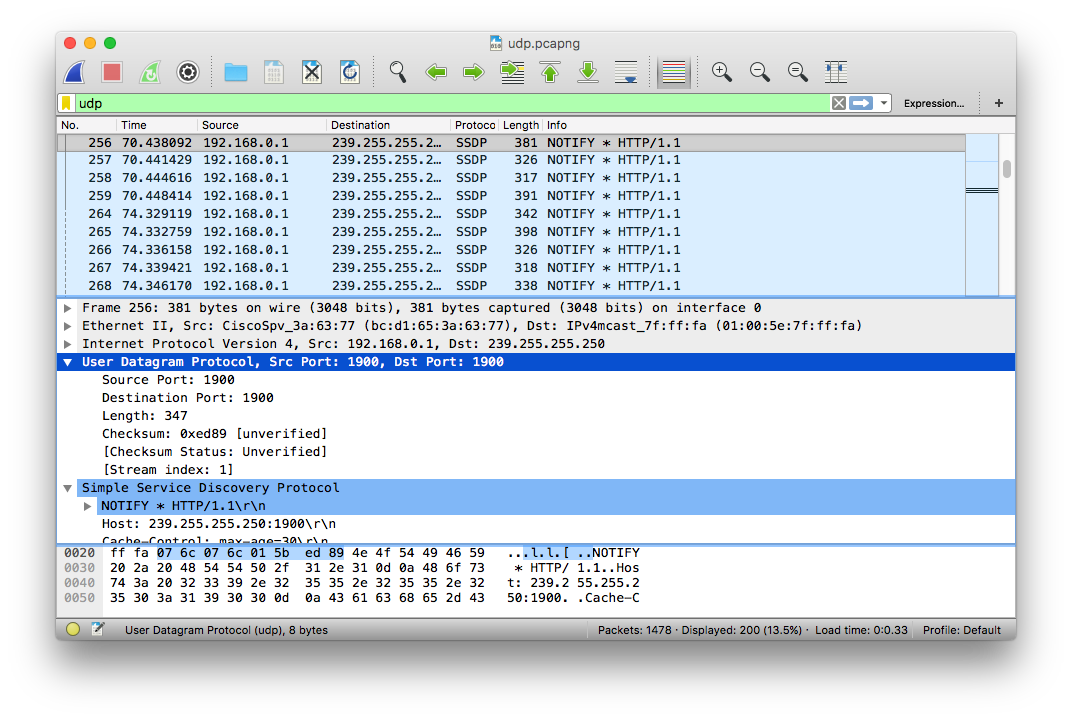
\includegraphics[width=\textwidth]{01}
		\end{figure}

	\item
		\textit{By consulting the displayed information in Wireshark’s packet content field for this packet, determine the length (in bytes) of each of the UDP header fields.}
		\par Each one of the fields in the UDP header is 2 bytes long.
		
		\begin{figure}[H]
		\centering
		\caption{Field size example (length)}
		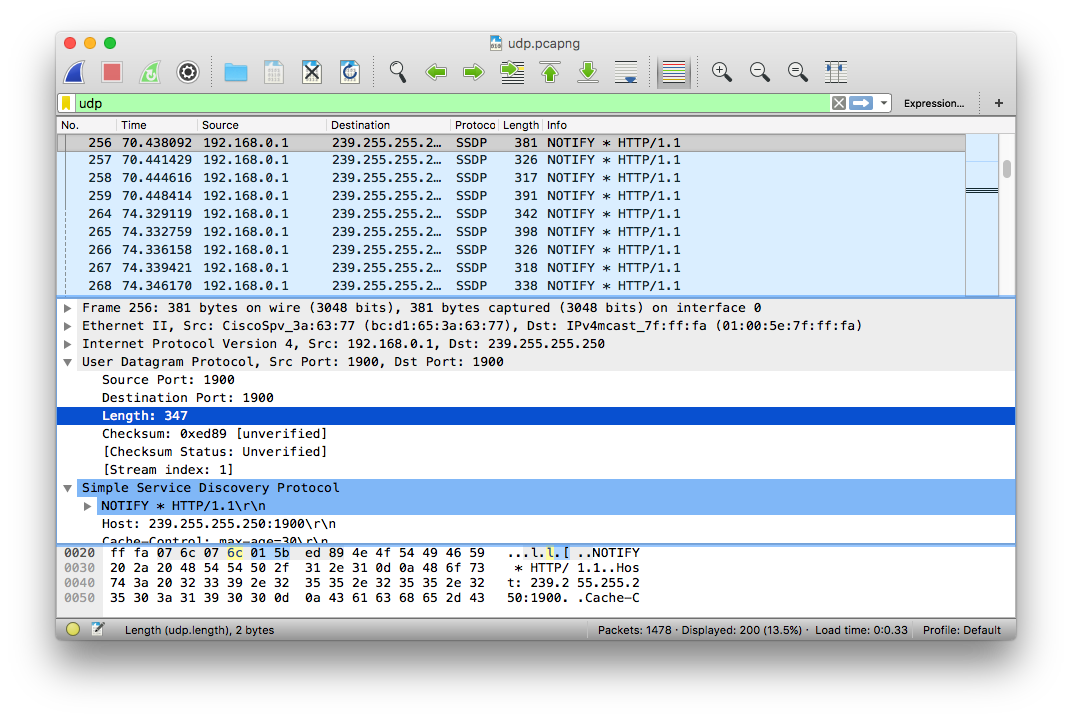
\includegraphics[width=\textwidth]{02}
		\end{figure}
	
	\item
		\textit{The value in the Length field is the length of what? (You can consult the text for this answer). Verify your claim with your captured UDP packet.}
		\par The value in the length field (347 bytes) is the sum of the header length (8 bytes) plus the SSDP data (339 bytes).
		
		\begin{figure}[H]
		\centering
		\caption{SSDP data length}
		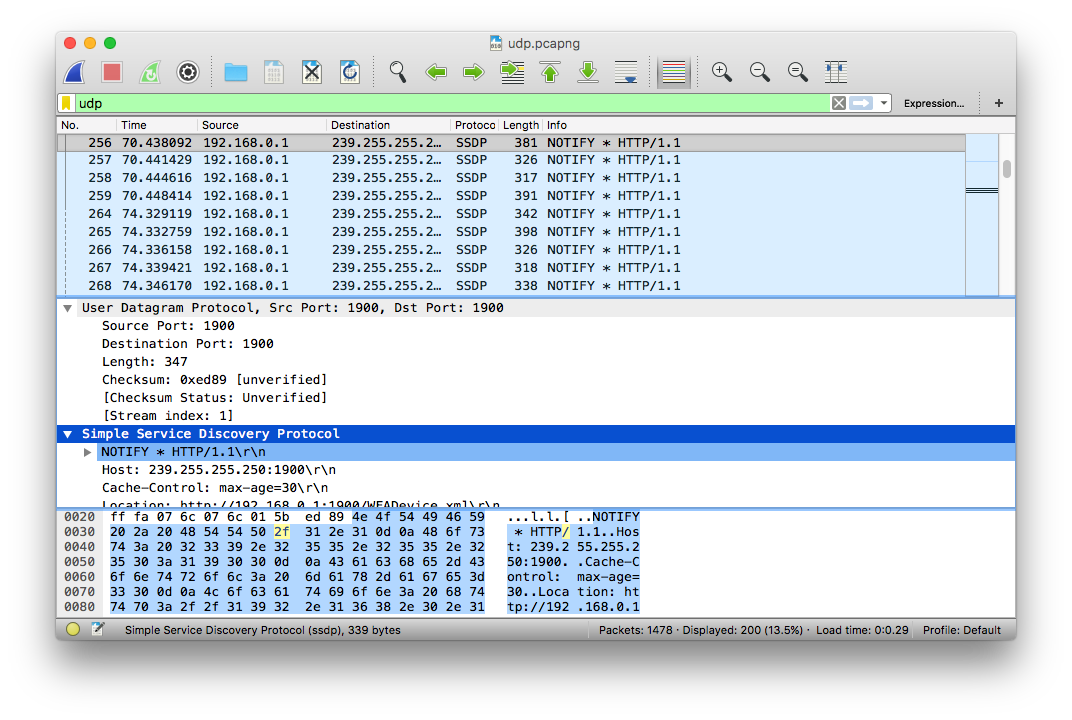
\includegraphics[width=\textwidth]{03}
		\end{figure}
		
	\item
		\textit{What is the maximum number of bytes that can be included in a UDP payload? (Hint: the answer to this question can be determined by your answer to 2. above)}
		\par The maximum number of bytes that can be included in a UDP payload is $2^{16}$ minus the number of bytes in the header (8). Therefore, 65535 – 8 = \textbf{65527} bytes.
		
	\item
		\textit{What is the largest possible source port number? (Hint: see the hint in 4.)}
		\par The largest possible source port number is $2^{16}$ = \textbf{65527}.
		
\pagebreak

	\item
		\textit{What is the protocol number for UDP? Give your answer in both hexadecimal and decimal notation. To answer this question, you’ll need to look into the Protocol field of the IP datagram containing this UDP segment (see Figure 4.13 in the text, and the discussion of IP header fields).}
		\par The protocol number for UDP is 0x11 hex, which translates to 17 in decimal.
		
		\begin{figure}[H]
		\centering
		\caption{UDP protocol number}
		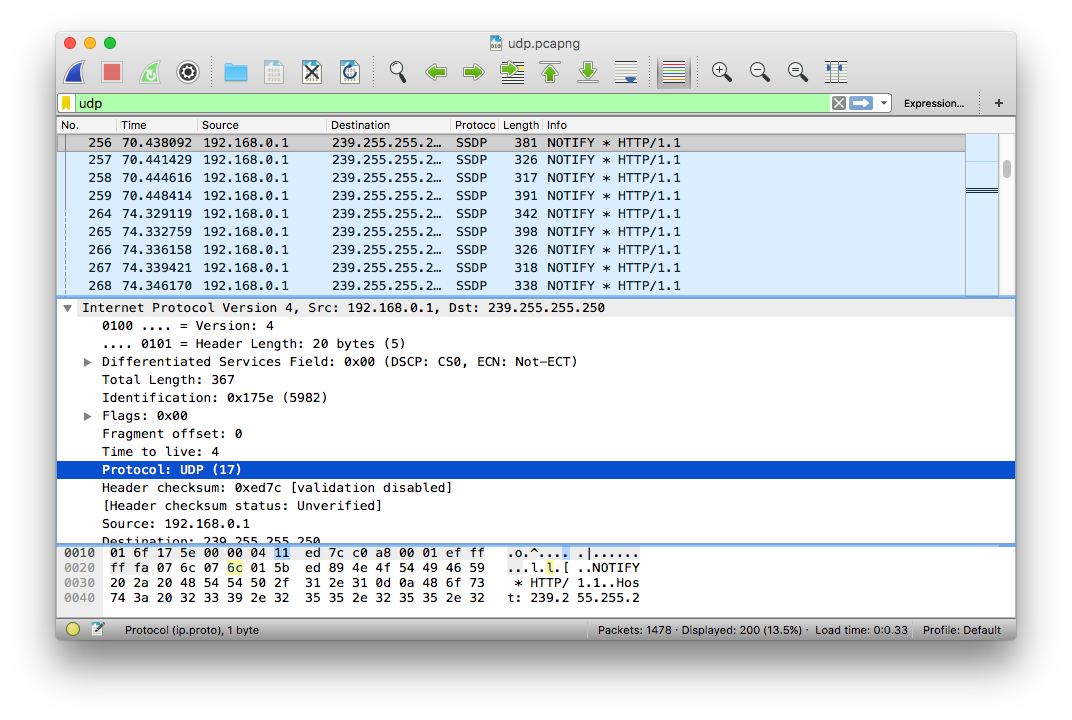
\includegraphics[width=\textwidth]{04}
		\end{figure}

	\item
		\textit{Examine a pair of UDP packets in which your host sends the first UDP packet and the second UDP packet is a reply to this first UDP packet. (Hint: for a second packet to be sent in response to a first packet, the sender of the first packet should be the destination of the second packet). Describe the relationship between the port numbers in the two packets.}
		\par The source port of the first UDP packet is the same as the destination port of the reply packet. Similarly, the destination port of the UDP packet that was sent is the same as the source port of the reply packet.
		
		\begin{figure}[H]
		\centering
		\caption{UDP packet sent by local host}
		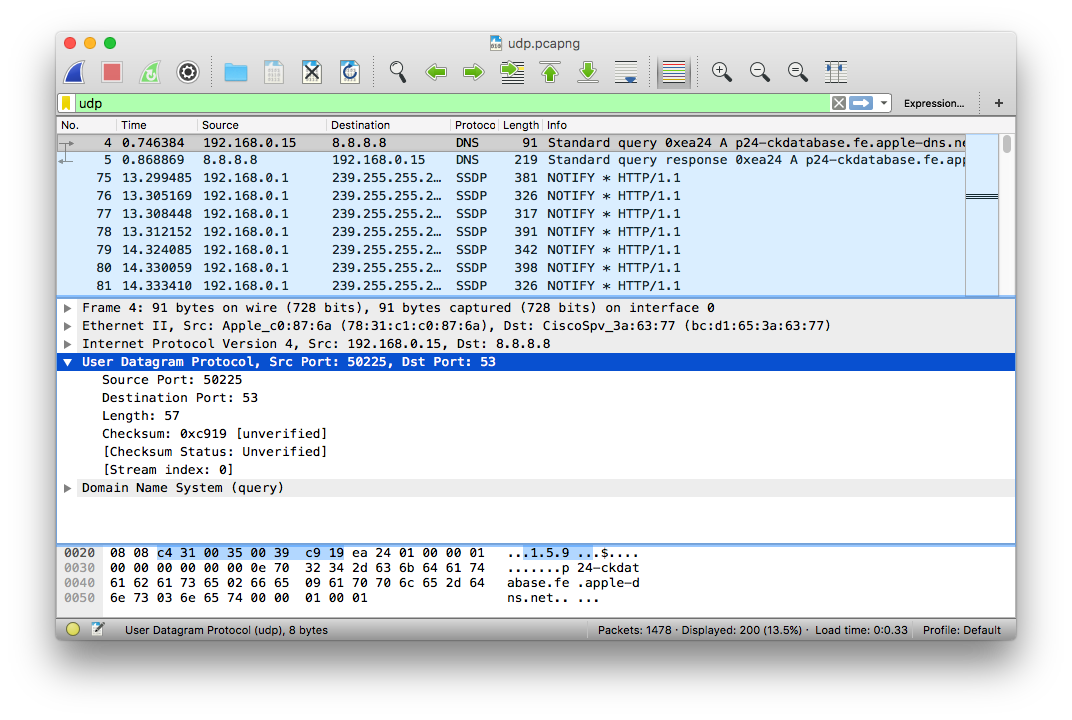
\includegraphics[width=380px]{05}
		\end{figure}
		
		\begin{figure}[H]
		\centering
		\caption{UDP reply packet received}
		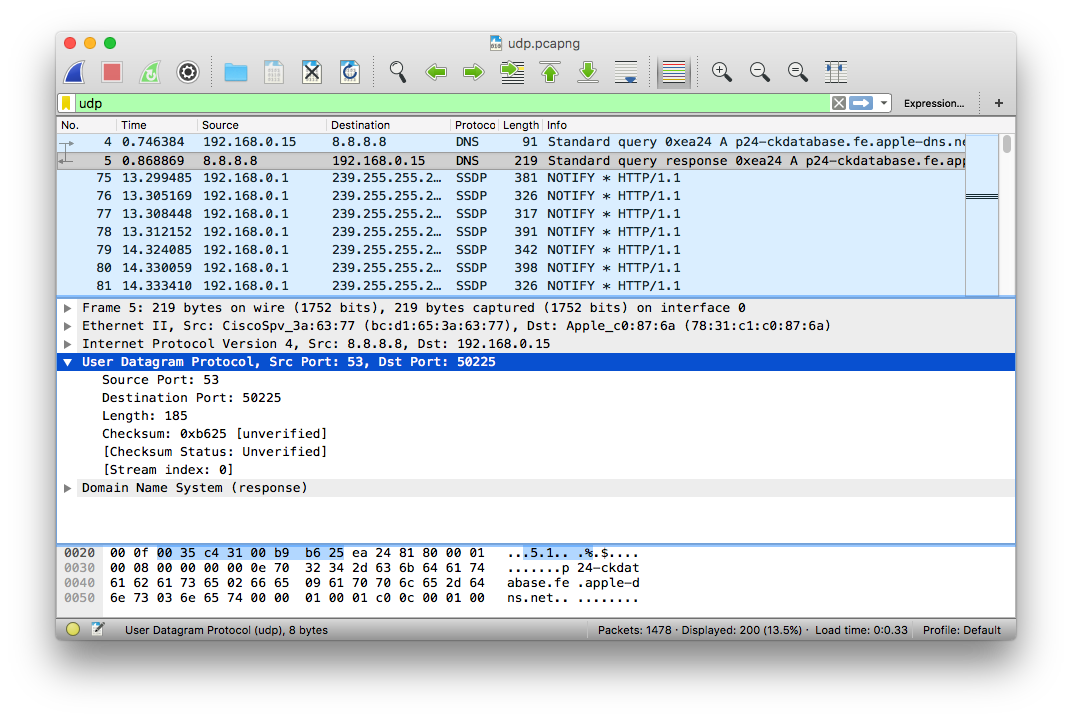
\includegraphics[width=380px]{06}
		\end{figure}

\end{itemize}

\end{document}
